JSON-Datei speichern

FA-E \ref{e-json-encodeing} %FA-E 47 JSON Encoding

JSON-Datei bearbeiten

FA-E \ref{e-json-decodeing} %FA-E 48 JSON Decoding

GUI anzeigen

FA-E \ref{e-gui} %FA-E 49 GUI

Szenarion Konfiguration erstellen und editieren

FA-E \ref{e-szenarioedit} %FA-E 50 Szenario Editor

Partie Konfiguration erstellen und editieren

FA-E \ref{e-partieedit} %FA-E 51 Partie Editor

Charakter Konfiguration erstellen und editieren

FA-E \ref{e-charedit} %FA-E 52 Charakter Editor

\begin{figure}
  \centering
  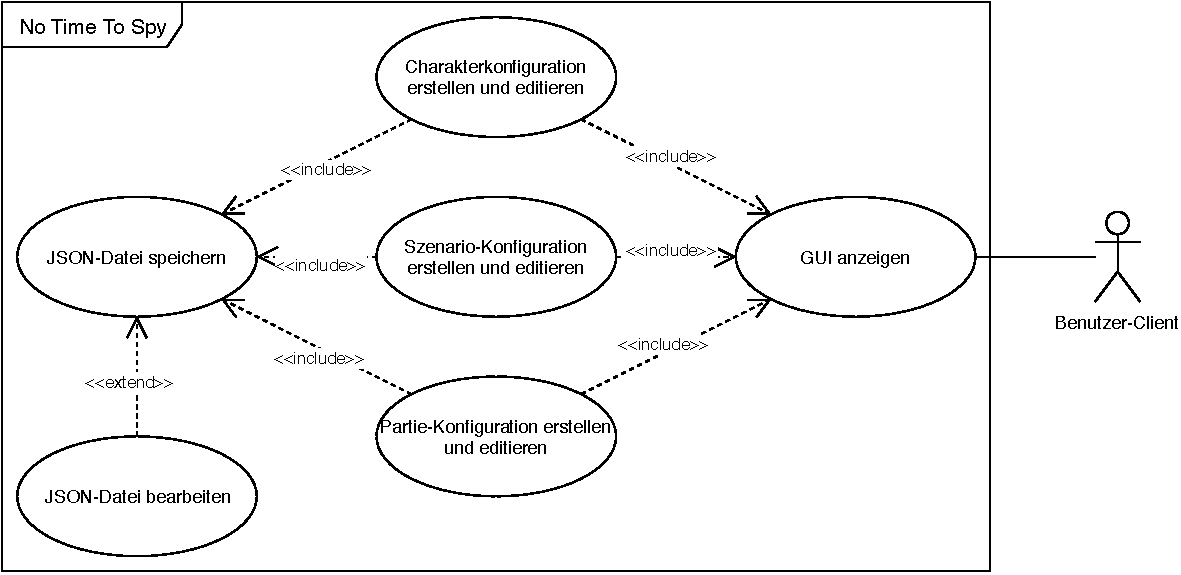
\includegraphics[width=\textwidth]{Meilenstein02/use_case_editor.pdf}
  \caption{Anwendungsfälle Editor}
\end{figure}